% Options for packages loaded elsewhere
\PassOptionsToPackage{unicode}{hyperref}
\PassOptionsToPackage{hyphens}{url}
\PassOptionsToPackage{dvipsnames,svgnames*,x11names*}{xcolor}
%
\documentclass[
  english,
  man,floatsintext]{apa6}
\usepackage{lmodern}
\usepackage{amssymb,amsmath}
\usepackage{ifxetex,ifluatex}
\ifnum 0\ifxetex 1\fi\ifluatex 1\fi=0 % if pdftex
  \usepackage[T1]{fontenc}
  \usepackage[utf8]{inputenc}
  \usepackage{textcomp} % provide euro and other symbols
\else % if luatex or xetex
  \usepackage{unicode-math}
  \defaultfontfeatures{Scale=MatchLowercase}
  \defaultfontfeatures[\rmfamily]{Ligatures=TeX,Scale=1}
\fi
% Use upquote if available, for straight quotes in verbatim environments
\IfFileExists{upquote.sty}{\usepackage{upquote}}{}
\IfFileExists{microtype.sty}{% use microtype if available
  \usepackage[]{microtype}
  \UseMicrotypeSet[protrusion]{basicmath} % disable protrusion for tt fonts
}{}
\makeatletter
\@ifundefined{KOMAClassName}{% if non-KOMA class
  \IfFileExists{parskip.sty}{%
    \usepackage{parskip}
  }{% else
    \setlength{\parindent}{0pt}
    \setlength{\parskip}{6pt plus 2pt minus 1pt}}
}{% if KOMA class
  \KOMAoptions{parskip=half}}
\makeatother
\usepackage{xcolor}
\IfFileExists{xurl.sty}{\usepackage{xurl}}{} % add URL line breaks if available
\IfFileExists{bookmark.sty}{\usepackage{bookmark}}{\usepackage{hyperref}}
\hypersetup{
  pdftitle={Epidemiologische situatie COVID-19 in Nederland - 17 juli 2021},
  pdfauthor={Marino van Zelst1},
  pdflang={en-EN},
  colorlinks=true,
  linkcolor=Maroon,
  filecolor=Maroon,
  citecolor=Blue,
  urlcolor=blue,
  pdfcreator={LaTeX via pandoc}}
\urlstyle{same} % disable monospaced font for URLs
\usepackage{graphicx,grffile}
\makeatletter
\def\maxwidth{\ifdim\Gin@nat@width>\linewidth\linewidth\else\Gin@nat@width\fi}
\def\maxheight{\ifdim\Gin@nat@height>\textheight\textheight\else\Gin@nat@height\fi}
\makeatother
% Scale images if necessary, so that they will not overflow the page
% margins by default, and it is still possible to overwrite the defaults
% using explicit options in \includegraphics[width, height, ...]{}
\setkeys{Gin}{width=\maxwidth,height=\maxheight,keepaspectratio}
% Set default figure placement to htbp
\makeatletter
\def\fps@figure{htbp}
\makeatother
\setlength{\emergencystretch}{3em} % prevent overfull lines
\providecommand{\tightlist}{%
  \setlength{\itemsep}{0pt}\setlength{\parskip}{0pt}}
\setcounter{secnumdepth}{-\maxdimen} % remove section numbering
% Make \paragraph and \subparagraph free-standing
\ifx\paragraph\undefined\else
  \let\oldparagraph\paragraph
  \renewcommand{\paragraph}[1]{\oldparagraph{#1}\mbox{}}
\fi
\ifx\subparagraph\undefined\else
  \let\oldsubparagraph\subparagraph
  \renewcommand{\subparagraph}[1]{\oldsubparagraph{#1}\mbox{}}
\fi
% Manuscript styling
\usepackage{upgreek}
\captionsetup{font=singlespacing,justification=justified}

% Table formatting
\usepackage{longtable}
\usepackage{lscape}
% \usepackage[counterclockwise]{rotating}   % Landscape page setup for large tables
\usepackage{multirow}		% Table styling
\usepackage{tabularx}		% Control Column width
\usepackage[flushleft]{threeparttable}	% Allows for three part tables with a specified notes section
\usepackage{threeparttablex}            % Lets threeparttable work with longtable

% Create new environments so endfloat can handle them
% \newenvironment{ltable}
%   {\begin{landscape}\begin{center}\begin{threeparttable}}
%   {\end{threeparttable}\end{center}\end{landscape}}
\newenvironment{lltable}{\begin{landscape}\begin{center}\begin{ThreePartTable}}{\end{ThreePartTable}\end{center}\end{landscape}}

% Enables adjusting longtable caption width to table width
% Solution found at http://golatex.de/longtable-mit-caption-so-breit-wie-die-tabelle-t15767.html
\makeatletter
\newcommand\LastLTentrywidth{1em}
\newlength\longtablewidth
\setlength{\longtablewidth}{1in}
\newcommand{\getlongtablewidth}{\begingroup \ifcsname LT@\roman{LT@tables}\endcsname \global\longtablewidth=0pt \renewcommand{\LT@entry}[2]{\global\advance\longtablewidth by ##2\relax\gdef\LastLTentrywidth{##2}}\@nameuse{LT@\roman{LT@tables}} \fi \endgroup}

% \setlength{\parindent}{0.5in}
% \setlength{\parskip}{0pt plus 0pt minus 0pt}

% \usepackage{etoolbox}
\makeatletter
\patchcmd{\HyOrg@maketitle}
  {\section{\normalfont\normalsize\abstractname}}
  {\section*{\normalfont\normalsize\abstractname}}
  {}{\typeout{Failed to patch abstract.}}
\patchcmd{\HyOrg@maketitle}
  {\section{\protect\normalfont{\@title}}}
  {\section*{\protect\normalfont{\@title}}}
  {}{\typeout{Failed to patch title.}}
\makeatother
\shorttitle{Dagelijkse rapportage}
\DeclareDelayedFloatFlavor{ThreePartTable}{table}
\DeclareDelayedFloatFlavor{lltable}{table}
\DeclareDelayedFloatFlavor*{longtable}{table}
\makeatletter
\renewcommand{\efloat@iwrite}[1]{\immediate\expandafter\protected@write\csname efloat@post#1\endcsname{}}
\makeatother
\usepackage{csquotes}
\ifxetex
  % Load polyglossia as late as possible: uses bidi with RTL langages (e.g. Hebrew, Arabic)
  \usepackage{polyglossia}
  \setmainlanguage[]{english}
\else
  \usepackage[shorthands=off,main=english]{babel}
\fi

\title{Epidemiologische situatie COVID-19 in Nederland - 17 juli 2021}
\author{Marino van Zelst\textsuperscript{1}}
\date{}


\affiliation{\vspace{0.5cm}\textsuperscript{1} Vragen over deze rapportage kunnen verstuurd worden aan Marino van Zelst, twitter.com/mzelst. E-mail: \href{mailto:j.m.vanzelst@uvt.nl}{\nolinkurl{j.m.vanzelst@uvt.nl}}}

\begin{document}
\maketitle

{
\hypersetup{linkcolor=}
\setcounter{tocdepth}{3}
\tableofcontents
}
\newpage

\hypertarget{samenvatting}{%
\section{Samenvatting}\label{samenvatting}}

\textbf{Samenvatting (op basis van GGD cijfers)}\\
Tot en met 2021-07-17 zijn er in Nederland in totaal 1788435 COVID-19 patiënten gemeld aan het RIVM. Tot nu toe zijn 30997 van de gemelde patiënten opgenomen in het ziekenhuis en 17775 mensen overleden.

\textbf{Gegevens t. o. v. gisteren}\\
Positief getest: 11134
Totaal: 1788435 (+ 11036 ivm -98 corr.)

Opgenomen: 16
Totaal: 30997 (+
16 ivm 0 corr.)

Overleden: 0
Totaal: 17775 (+
0 ivm 0 corr.)

\textbf{Update met betrekking tot ziekenhuis-gegevens (data NICE)}

Patiënten verpleegafdeling\\
Bevestigd: 1 Verdacht: 1

Patiënten IC\\
Bevestigd: 1 Verdacht: 0

\textbf{Data}\\
Een databestand met de cumulatieve aantallen per gemeente per dag van gemelde COVID-19 patiënten, in het ziekenhuis opgenomen COVID-19 patiënten en overleden COVID-19 patiënten is \href{https://data.rivm.nl/geonetwork/srv/dut/catalog.search\#/metadata/1c0fcd57-1102-4620-9cfa-441e93ea5604}{hier} te vinden. Een databestand met karakteristieken van elke positief geteste COVID-19 patiënt in Nederland is \href{https://data.rivm.nl/geonetwork/srv/dut/catalog.search\#/metadata/2c4357c8-76e4-4662-9574-1deb8a73f724?tab=relations}{hier} te vinden. Alle gegevens die voor dit rapport gebruikt worden zijn te vinden in de \href{https://github.com/mzelst/covid-19}{Github repository}.

\newpage

\hypertarget{covid-19-meldingen-in-de-afgelopen-vier-weken}{%
\section{COVID-19 meldingen in de afgelopen vier weken}\label{covid-19-meldingen-in-de-afgelopen-vier-weken}}

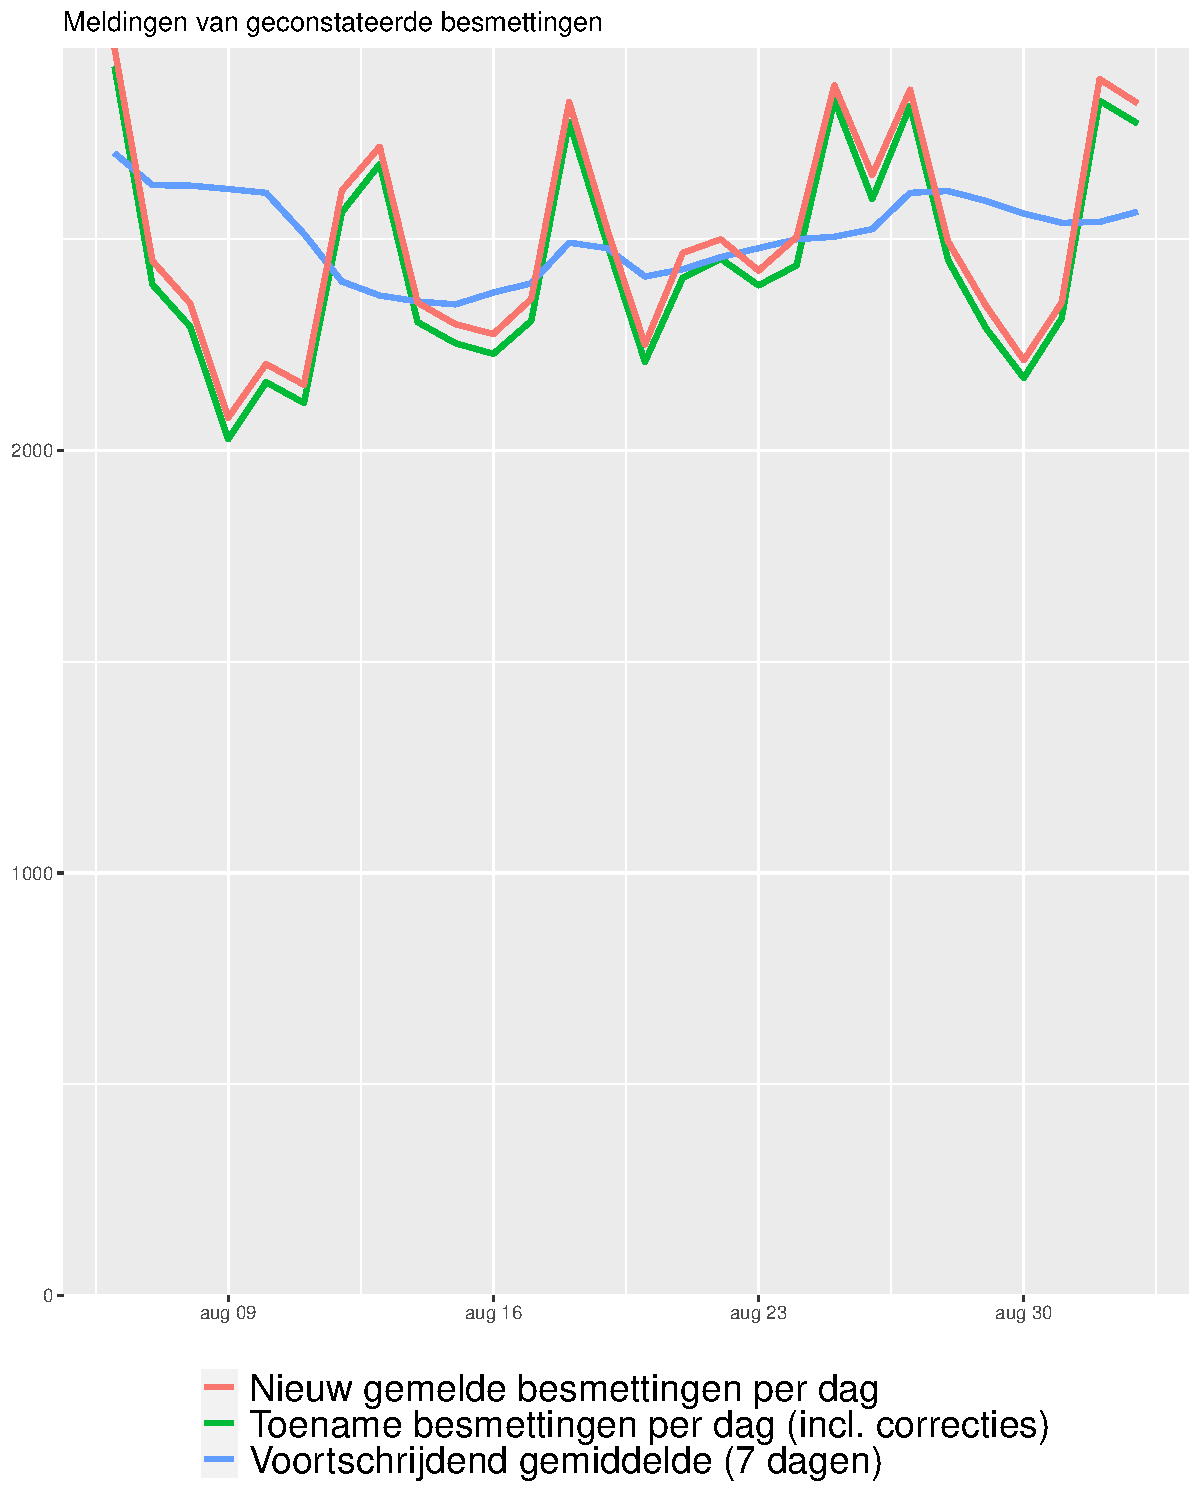
\includegraphics{daily_report_files/figure-latex/Gemelde besmettingen-1.pdf}

\newpage

\hypertarget{kaart-met-covid-19-meldingen-per-gemeente-sinds-gisteren}{%
\section{Kaart met COVID-19 meldingen per gemeente sinds gisteren}\label{kaart-met-covid-19-meldingen-per-gemeente-sinds-gisteren}}

\begin{figure}
\centering
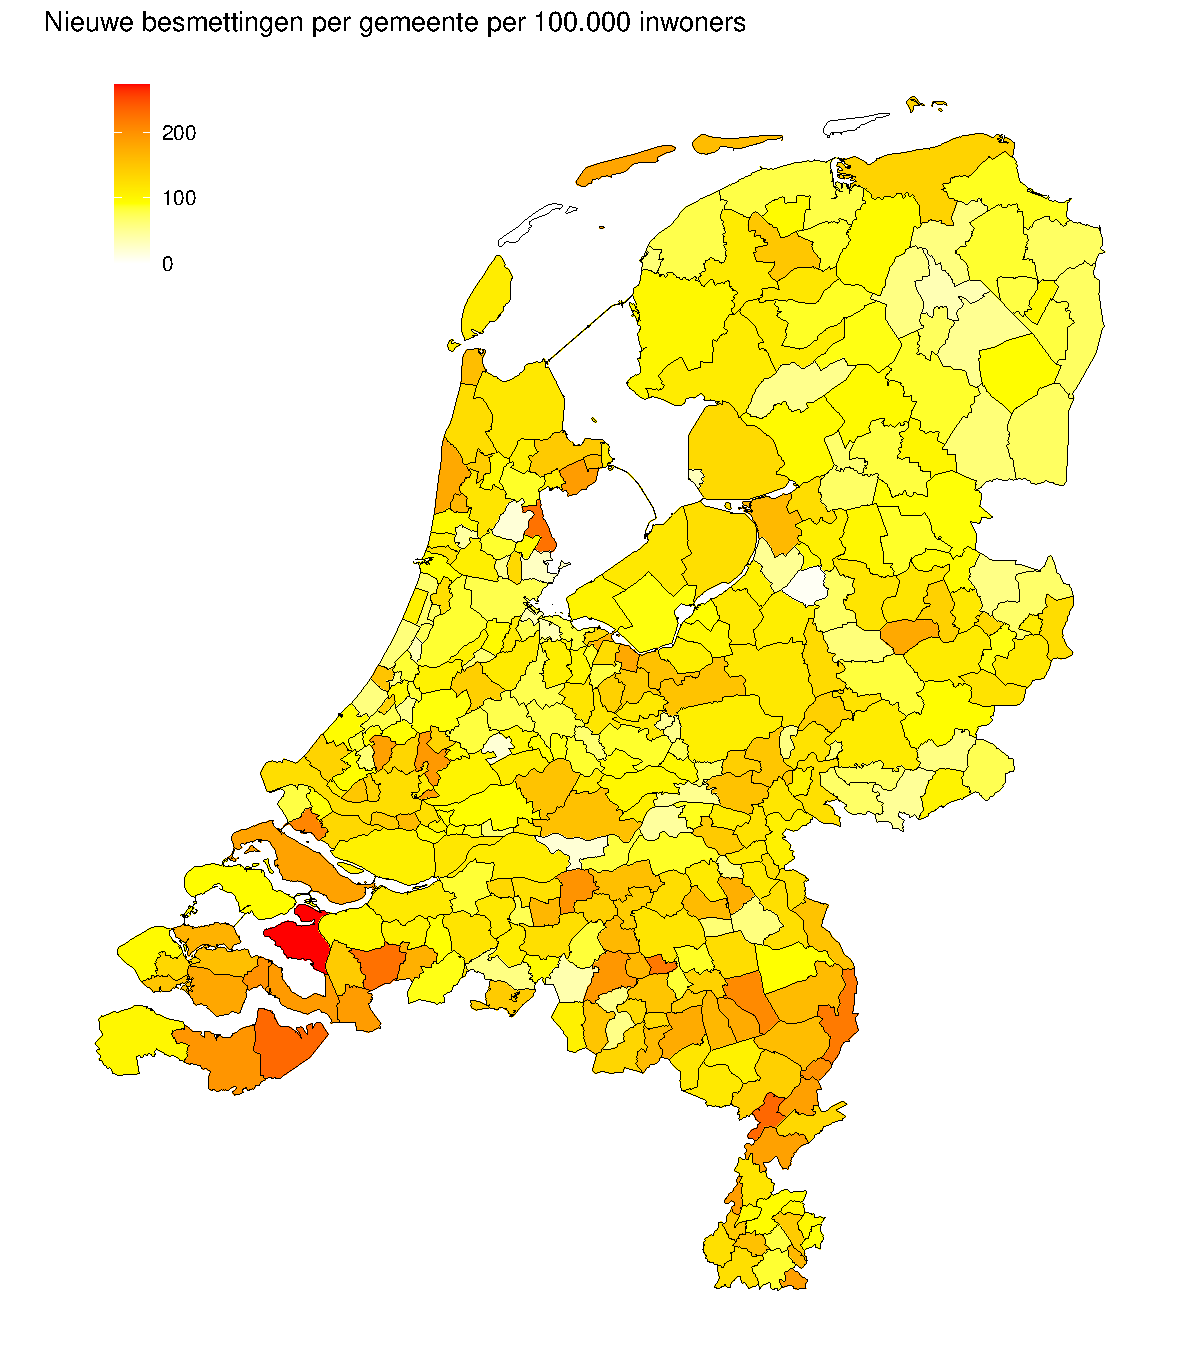
\includegraphics{daily_report_files/figure-latex/Gemeentes - sinds gisteren-1.pdf}
\caption{(\#Gemeentes - sinds gisteren) Aantal, sinds gisteren, bij de GGD'en gemelde COVID-19 patiënten per 100.000 inwoners per gemeente}
\end{figure}

\newpage

\hypertarget{kaart-met-covid-19-meldingen-per-gemeente-in-de-afgelopen-week}{%
\section{Kaart met COVID-19 meldingen per gemeente in de afgelopen week}\label{kaart-met-covid-19-meldingen-per-gemeente-in-de-afgelopen-week}}

\begin{figure}
\centering
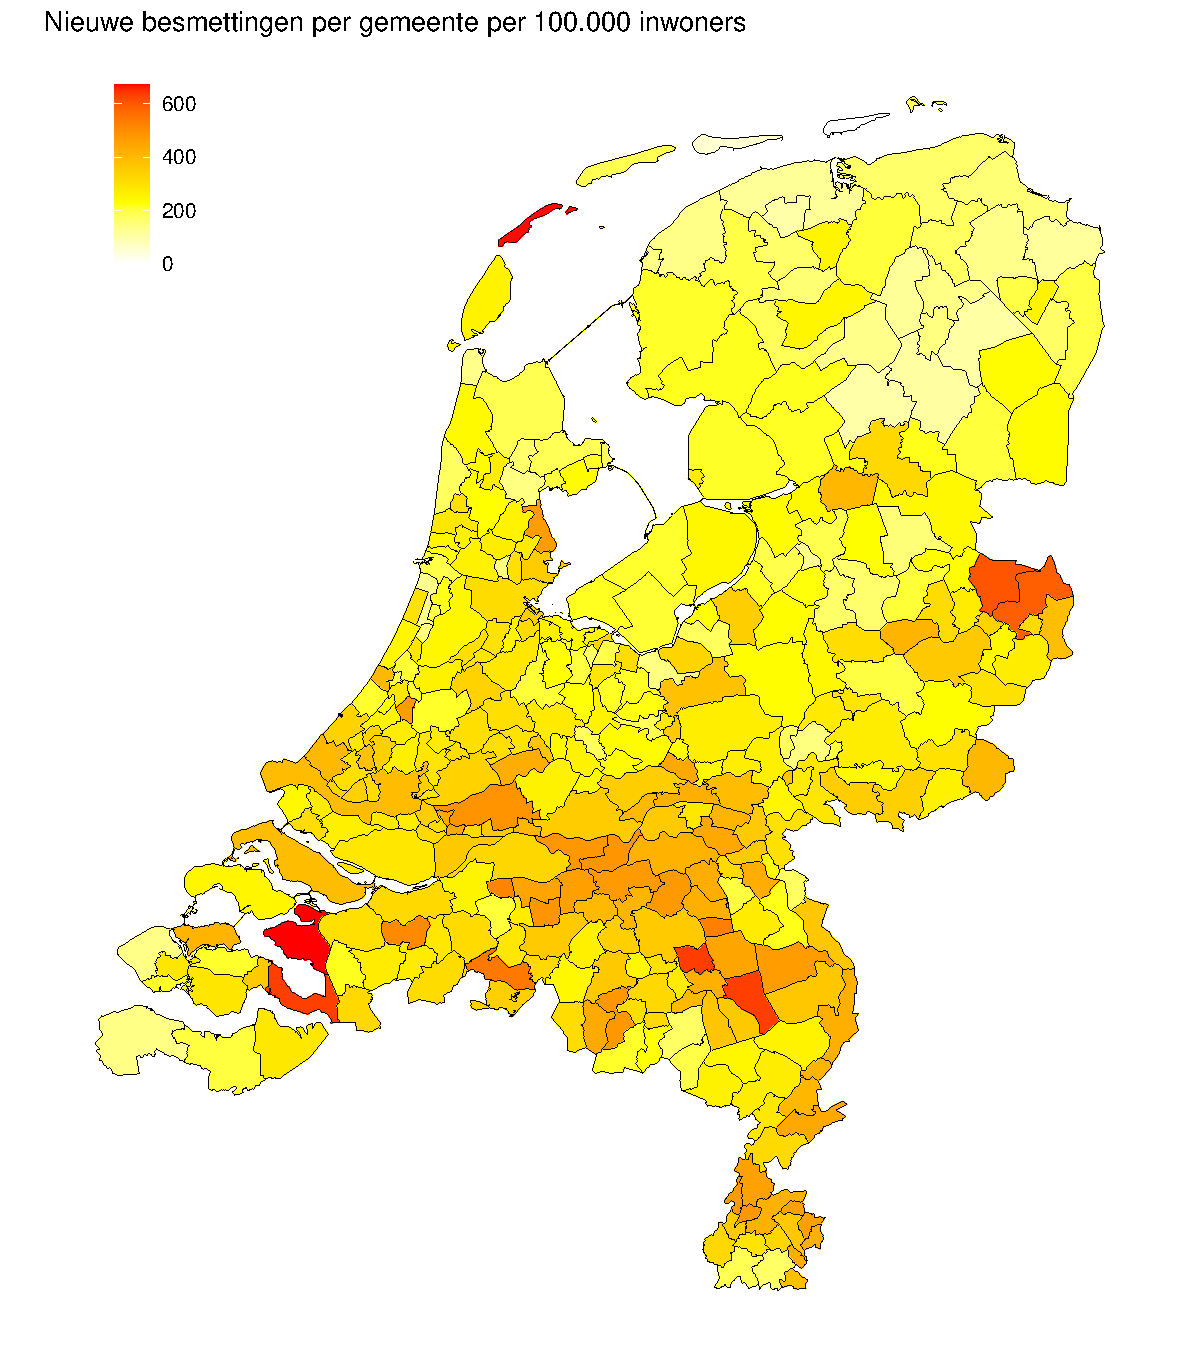
\includegraphics{daily_report_files/figure-latex/Gemeentes - Sinds vorige week-1.pdf}
\caption{(\#Gemeentes - Sinds vorige week) Aantal in de afgelopen week bij de GGD'en gemelde COVID-19 patiënten per 100.000 inwoners per gemeente.}
\end{figure}

\newpage

\hypertarget{aantal-covid-19-meldingen-per-provincie-in-de-afgelopen-twee-weken}{%
\section{Aantal COVID-19 meldingen per provincie in de afgelopen twee weken}\label{aantal-covid-19-meldingen-per-provincie-in-de-afgelopen-twee-weken}}

\begin{table}
\centering
\begin{threeparttable}
\begin{tabular}{lrrrrrr}
\toprule
\multicolumn{1}{c}{ } & \multicolumn{2}{c}{Besmettingen} & \multicolumn{2}{c}{Ziekenhuisopnames} & \multicolumn{2}{c}{Overleden} \\
\cmidrule(l{3pt}r{3pt}){2-3} \cmidrule(l{3pt}r{3pt}){4-5} \cmidrule(l{3pt}r{3pt}){6-7}
Provincie & Totaal & /100000 & Totaal & /100000 & Totaal & /100000\\
\midrule
Drenthe & 1359 & 274.1 & 3 & 0.6 & 0 & 0.0\\
Flevoland & 1331 & 309.0 & 4 & 0.9 & 0 & 0.0\\
Fryslân & 2183 & 334.9 & 4 & 0.6 & 1 & 0.2\\
Gelderland & 9487 & 451.8 & 11 & 0.5 & 1 & 0.0\\
Groningen & 5374 & 915.7 & 1 & 0.2 & 0 & 0.0\\
Limburg & 3376 & 302.6 & 6 & 0.5 & 1 & 0.1\\
Noord-Brabant & 13315 & 516.4 & 6 & 0.2 & 0 & 0.0\\
Noord-Holland & 25106 & 869.2 & 30 & 1.0 & 7 & 0.2\\
Overijssel & 5504 & 471.4 & 6 & 0.5 & 0 & 0.0\\
Utrecht & 10285 & 754.9 & 9 & 0.7 & 1 & 0.1\\
Zeeland & 963 & 249.6 & 7 & 1.8 & 0 & 0.0\\
Zuid-Holland & 22261 & 596.6 & 21 & 0.6 & 8 & 0.2\\
\bottomrule
\end{tabular}
\begin{tablenotes}
\item \textit{Note: } 
\item Aantal bij de GGD’en gemelde COVID-19 patiënten, in het ziekenhuis opgenomen COVID-19 patiënten en overleden COVID-19 patiënten per provincie van 03 juli t/m 17 juli 10:00 uur, totaal en per 100.000 inwoners
\end{tablenotes}
\end{threeparttable}
\end{table}

\newpage

\hypertarget{aantal-covid-19-meldingen-per-ggd-in-de-afgelopen-twee-weken}{%
\section{Aantal COVID-19 meldingen per GGD in de afgelopen twee weken}\label{aantal-covid-19-meldingen-per-ggd-in-de-afgelopen-twee-weken}}

\begin{table}
\centering\begingroup\fontsize{10}{12}\selectfont

\begin{threeparttable}
\begin{tabular}{lrrrrrr}
\toprule
\multicolumn{1}{c}{ } & \multicolumn{2}{c}{Besmettingen} & \multicolumn{2}{c}{Ziekenhuisopnames} & \multicolumn{2}{c}{Overleden} \\
\cmidrule(l{3pt}r{3pt}){2-3} \cmidrule(l{3pt}r{3pt}){4-5} \cmidrule(l{3pt}r{3pt}){6-7}
GGD & Totaal & /100000 & Totaal & /100000 & Totaal & /100000\\
\midrule
Dienst Gezondheid \& Jeugd ZHZ & 1669 & 361.5 & 1 & 0.2 & 1 & 0.2\\
GGD Amsterdam & 14259 & 1331.9 & 17 & 1.6 & 5 & 0.5\\
GGD Brabant-Zuidoost & 3922 & 499.2 & 1 & 0.1 & 0 & 0.0\\
GGD Drenthe & 1340 & 270.1 & 3 & 0.6 & 0 & 0.0\\
GGD Flevoland & 1319 & 306.0 & 4 & 0.9 & 0 & 0.0\\
GGD Fryslân & 2232 & 342.2 & 4 & 0.6 & 1 & 0.2\\
GGD Gelderland-Zuid & 3175 & 561.8 & 1 & 0.2 & 1 & 0.2\\
GGD Gooi en Vechtstreek & 1931 & 743.9 & 4 & 1.5 & 0 & 0.0\\
GGD Groningen & 5332 & 908.5 & 1 & 0.2 & 0 & 0.0\\
GGD Haaglanden & 6169 & 548.6 & 6 & 0.5 & 1 & 0.1\\
GGD Hart voor Brabant & 4701 & 434.5 & 3 & 0.3 & 0 & 0.0\\
GGD Hollands-Midden & 4870 & 596.4 & 1 & 0.1 & 1 & 0.1\\
GGD Hollands-Noorden & 2889 & 432.7 & 5 & 0.7 & 0 & 0.0\\
GGD IJsselland & 2111 & 393.8 & 1 & 0.2 & 0 & 0.0\\
GGD Kennemerland & 4076 & 738.4 & 5 & 0.9 & 2 & 0.4\\
GGD Limburg-Noord & 1549 & 296.4 & 4 & 0.8 & 1 & 0.2\\
GGD Noord- en Oost-Gelderland & 3490 & 419.0 & 2 & 0.2 & 0 & 0.0\\
GGD Regio Utrecht & 10267 & 1625.1 & 9 & 1.4 & 1 & 0.2\\
GGD Rotterdam-Rijnmond & 9546 & 700.4 & 13 & 1.0 & 5 & 0.4\\
GGD Twente & 3373 & 253.7 & 5 & 0.4 & 0 & 0.0\\
GGD West-Brabant & 4710 & 661.6 & 2 & 0.3 & 0 & 0.0\\
GGD Zaanstreek/Waterland & 2022 & 595.6 & 0 & 0.0 & 0 & 0.0\\
GGD Zeeland & 963 & 249.6 & 6 & 1.6 & 0 & 0.0\\
GGD Zuid-Limburg & 1826 & 307.9 & 2 & 0.3 & 0 & 0.0\\
Veiligheids- en Gezondheidsregio Gelderland-Midden & 2803 & 398.8 & 8 & 1.1 & 0 & 0.0\\
\bottomrule
\end{tabular}
\begin{tablenotes}
\item \textit{Note: } 
\item Aantal bij de GGD’en gemelde COVID-19 patiënten, in het ziekenhuis opgenomen COVID-19 patiënten en overleden COVID-19 patiënten per GGD van 03 juli t/m 17 juli 10:00 uur, totaal en per 100.000 inwoners
\end{tablenotes}
\end{threeparttable}
\endgroup{}
\end{table}

\newpage

\hypertarget{ziekenhuisopnames-nice-in-de-afgelopen-twee-weken}{%
\section{Ziekenhuisopnames (NICE) in de afgelopen twee weken}\label{ziekenhuisopnames-nice-in-de-afgelopen-twee-weken}}

\begin{table}
\centering\begingroup\fontsize{10}{12}\selectfont

\begin{threeparttable}
\begin{tabular}{lrrrrrr}
\toprule
\multicolumn{1}{c}{ } & \multicolumn{2}{c}{Aanwezig} & \multicolumn{2}{c}{Opnames} & \multicolumn{2}{c}{Overleden} \\
\cmidrule(l{3pt}r{3pt}){2-3} \cmidrule(l{3pt}r{3pt}){4-5} \cmidrule(l{3pt}r{3pt}){6-7}
Leeftijd & Kliniek & IC & Kliniek & IC & Kliniek & IC\\
\midrule
<20 & 35 & 0 & 30 & -1 & 0 & 0\\
20 - 24 & 9 & 0 & 19 & 1 & 0 & 0\\
25 - 29 & 13 & 0 & 15 & 2 & 0 & 0\\
30 - 34 & 9 & 3 & 18 & 3 & 0 & 0\\
35 - 39 & 10 & 1 & 15 & 0 & 0 & 0\\
40 - 44 & 12 & 4 & 10 & 3 & 0 & 1\\
45 - 49 & 13 & 8 & 16 & 7 & 0 & 0\\
50 - 54 & 30 & 14 & 11 & 9 & 0 & 1\\
55 - 59 & 23 & 10 & 14 & 6 & 0 & 3\\
60 - 64 & 17 & 11 & 16 & 0 & 2 & 3\\
65 - 69 & 19 & 13 & 8 & 2 & 3 & 4\\
70 - 74 & 23 & 14 & 9 & 3 & 0 & 3\\
75 - 79 & 21 & 2 & 5 & 3 & 1 & 1\\
80 - 84 & 17 & 1 & 9 & 0 & 3 & 0\\
85 - 89 & 11 & 0 & 0 & 0 & 5 & 0\\
>90 & 10 & 0 & 5 & 0 & 0 & 0\\
\bottomrule
\end{tabular}
\begin{tablenotes}
\item \textit{Note: } 
\item Aantal bij NICE gemelde COVID-19 patiënten: in het ziekenhuis aanwezige COVID-19 patiënten, opnames, en overleden COVID-19 patiënten in het ziekenhuis van 03 juli t/m 17 juli 15:15 uur
\end{tablenotes}
\end{threeparttable}
\endgroup{}
\end{table}

\newpage

\hypertarget{leeftijdsverdeling-en-man-vrouwverdeling-van-covid-19-patiuxebnten-in-de-afgelopen-twee-weken}{%
\section{Leeftijdsverdeling en man-vrouwverdeling van COVID-19 patiënten in de afgelopen twee weken}\label{leeftijdsverdeling-en-man-vrouwverdeling-van-covid-19-patiuxebnten-in-de-afgelopen-twee-weken}}

\begin{table}
\centering\begingroup\fontsize{11}{13}\selectfont

\begin{threeparttable}
\begin{tabular}{lrrrrrr}
\toprule
\multicolumn{1}{c}{ } & \multicolumn{2}{c}{Besmettingen} & \multicolumn{2}{c}{Ziekenhuisopnames} & \multicolumn{2}{c}{Overleden} \\
\cmidrule(l{3pt}r{3pt}){2-3} \cmidrule(l{3pt}r{3pt}){4-5} \cmidrule(l{3pt}r{3pt}){6-7}
Leeftijdsgroep & Totaal & \% & Totaal & \% & Totaal & \%\\
\midrule
0-9 & 1870 & 1.9 & 3 & 2.8 & 0 & 0.0\\
10-19 & 25479 & 25.3 & 10 & 9.3 & 0 & 0.0\\
20-29 & 49887 & 49.6 & 25 & 23.1 & 0 & 0.0\\
30-39 & 9905 & 9.9 & 11 & 10.2 & 0 & 0.0\\
40-49 & 5595 & 5.6 & 4 & 3.7 & 0 & 0.0\\
50-59 & 5513 & 5.5 & 19 & 17.6 & 3 & 16.7\\
60-69 & 1606 & 1.6 & 13 & 12.0 & 4 & 22.2\\
70-79 & 426 & 0.4 & 12 & 11.1 & 6 & 33.3\\
80-89 & 207 & 0.2 & 10 & 9.3 & 2 & 11.1\\
90+ & 55 & 0.1 & 1 & 0.9 & 3 & 16.7\\
\bottomrule
\end{tabular}
\begin{tablenotes}
\item[1] Leeftijdsverdeling van bij de GGD’en gemelde COVID-19 patiënten, in het ziekenhuis opgenomen COVID-19 patiënten en overleden COVID-19 patiënten van 03 juli t/m 17 juli 10:00 uur.
\end{tablenotes}
\end{threeparttable}
\endgroup{}
\end{table}

\newpage

\begin{table}
\centering\begingroup\fontsize{11}{13}\selectfont

\begin{threeparttable}
\begin{tabular}{lrrrrrr}
\toprule
\multicolumn{1}{c}{ } & \multicolumn{2}{c}{Besmettingen} & \multicolumn{2}{c}{Ziekenhuisopnames} & \multicolumn{2}{c}{Overleden} \\
\cmidrule(l{3pt}r{3pt}){2-3} \cmidrule(l{3pt}r{3pt}){4-5} \cmidrule(l{3pt}r{3pt}){6-7}
Geslacht & Totaal & \% & Totaal & \% & Totaal & \%\\
\midrule
Vrouw & 49542 & 49.3 & 58 & 53.7 & 8 & 42.1\\
Man & 51002 & 50.7 & 50 & 46.3 & 11 & 57.9\\
Onbekend & 0 & 0.0 & 0 & 0.0 & 0 & 0.0\\
\bottomrule
\end{tabular}
\begin{tablenotes}
\item \textit{Note: } 
\item Man-vrouwverdeling van bij de GGD’en gemelde COVID-19 patiënten, in het ziekenhuis opgenomen COVID-19 patiënten en overleden COVID-19 patiënten van 03 juli t/m 17 juli 10:00 uur.
\end{tablenotes}
\end{threeparttable}
\endgroup{}
\end{table}
\newpage


\end{document}
